
%(BEGIN_QUESTION)
% Copyright 2010, Tony R. Kuphaldt, released under the Creative Commons Attribution License (v 1.0)
% This means you may do almost anything with this work of mine, so long as you give me proper credit

Examine this pneumatic signal relay cut-away diagram:

$$\includegraphics[width=15.5cm]{i04352x01.eps}$$

Identify the mathematical expression that best describes this relay's operation, assuming that the spring adjustment screw ($K$) {\it pushes down} on the spring to compress it rather than pulls up on the spring to stretch it:

\begin{itemize}
\item{} $A = 0.5E - K$
\vskip 5pt
\item{} $A = K - 0.5E$
\vskip 5pt
\item{} $A = 2E - K$
\vskip 5pt
\item{} $A = K + 2E$
\vskip 5pt
\item{} $A = \sqrt{E} - K$
\vskip 5pt
\item{} $A = K - 2E$
\vskip 5pt
\item{} $A = 0.5E + K$
\vskip 5pt
\item{} $A = \sqrt{E} + K$
\end{itemize}

Also, identify whether this relay employs the {\it force-balance} principle or the {\it motion-balance} principle.  Hint: assume the output tube ($A$) dead-ends at a pressure gauge, so there is no air flow when the relay has achieved a ``balanced'' (equilibrium) condition.

\underbar{file i04352}
%(END_QUESTION)





%(BEGIN_ANSWER)

I recommend assigning half credit for the correct mathematical expression, and half credit for the correct identification of balance principle.

\vskip 10pt

Best description of relay function:  $A = 0.5E + K$

\vskip 10pt

This is a {\it force-balance} mechanism.

%(END_ANSWER)





%(BEGIN_NOTES)

{\bf This question is intended for exams only and not worksheets!}.

%(END_NOTES)


